\section{Setup of CAN-interface}
t.b.d.

\subsection{Connection Scheme}
The CAN-bus shall be connected to the Gleisbox as depicted in figure~\ref{fig:mobilestation2_din10}. The pin 1 (power supply) does not have to be connected.


\begin{figure}[h!]
	\centering
	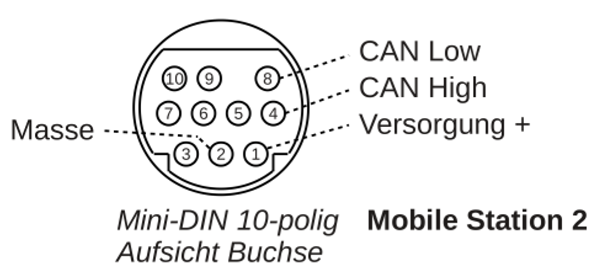
\includegraphics[width=1.00\linewidth]{../figures/mobilestation2_din10.png}
	\caption{Pinout canbus.}
	\label{fig:mobilestation2_din10}
\end{figure}

\subsection{Oscillator Settings}



\begin{figure}[h!]
	\centering
	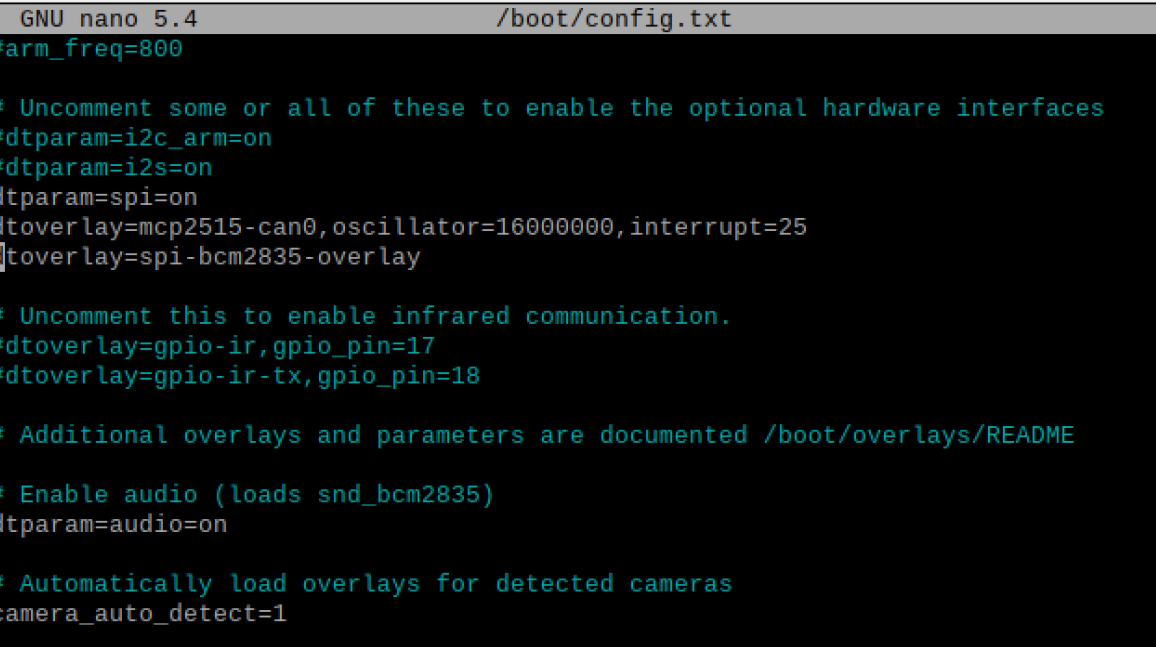
\includegraphics[width=1.00\linewidth]{../figures/oscillatorSettingsConfigTxt.png}
	\caption{Pi Oscillator settings.}
	\label{fig:oscillatorSettingsConfigTxt}
\end{figure}

sudo ip link set can0 up type can bitrate 250000


\subsection{Rocrail Server Settings}



\begin{figure}[h!]
	\centering
	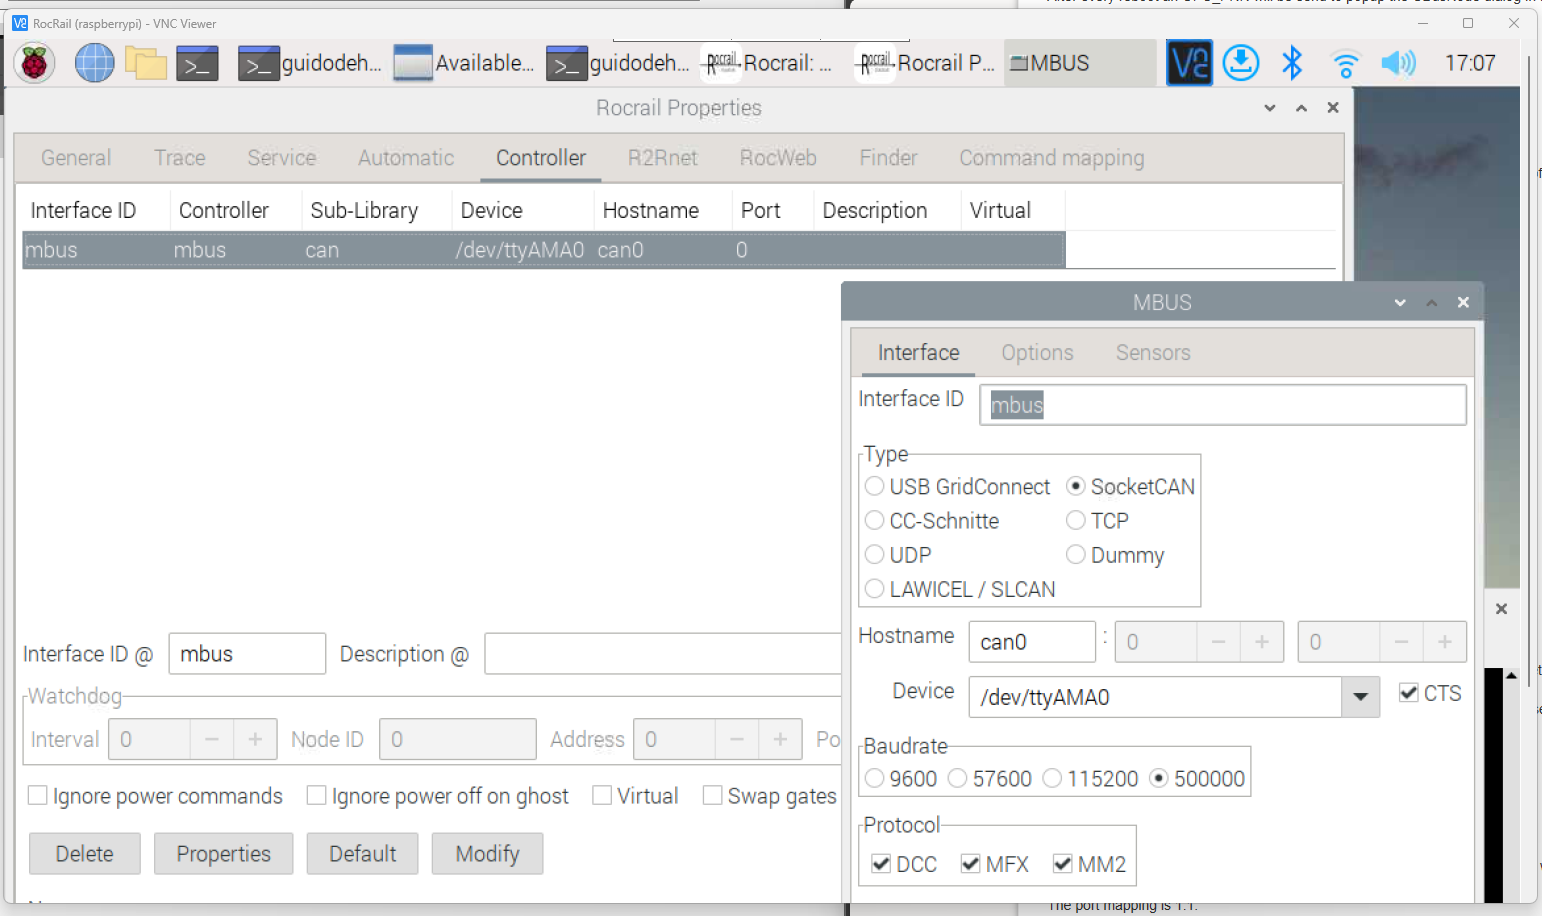
\includegraphics[width=1.00\linewidth]{../figures/rocrailServerSettings.png}
	\caption{rocrailServerSettings.}
	\label{fig:rocrailServerSettings}
\end{figure}


